\chapter{The geomorphic orientation system}\label{ch-geomorphic}

\section{Introduction}

\emph{Geomorphic}\footnote{Terminology following \citet{Bickel1997Spatial}.} spatial expressions present an absolute system, relying on the features of the landscape. The anchor of this system is the inclination of the steep hills that shape so many aspects of life in the Kiranti area (see also Figure \ref{tumok-path}). The system is absolute, as the directions of uphill and downhill are grounded in the environment and do not depend upon the orientation of the speaker or any other object. It can also be deictic, however, because these directions are in many cases defined from the perspective of the utterance context. 

As a distinctive  feature of Kiranti languages, geomorphic systems have been the subject of a number of studies, for example by \citet{Allen1972The-vertical} for Thulung, \citet{Bickel1994Mapping, Bickel1999Cultural, Bickel1997Spatial, Bickel2001Deictic} for Belhare, \citet{Gaenszle1999Travelling} for Mewahang, \citet{Dirksmeyer2008Spatial} for Chintang.\footnote{Geomorphic orientation systems are, however, not unique to Kiranti languages. Another famous example is the Mayan language Tzeltal \citep{Brownetal1993Uphill}.} What makes Kiranti languages special is that this topography-based deixis is also used for micro-location, for instance for distinguishing two glasses on a table or two branches on a tree. 

There are two mapping systems, large-scale, defined by the global inclination of the Himalayas (roughly, \rede{uphill} can be equated with \rede{north} in this mapping system), and small-scale, defined by the cline of individual hills. As also pointed out for Belhare by \citet[55]{Bickel1997Spatial}, the large-scale abstraction ignores the cline of individual hills, and the small-scale abstraction ignores horizontal planes on a hill. To give an example for the large-scale abstraction: speakers refer to any location outside the Himalayas (even as far away as Europe or America) as \rede{downhill}. To give an example for the small-scale abstraction: rooms on the same level of the house are divided into \rede{uphill} and \rede{downhill} rooms, depending on which side of the house faces the hill on which it is located. The latter can be extended to refer to \rede{up} and \rede{down}, too (as in \rede{up into the sky}). 
%\footnote{This kind of spatial expression is both geomorphic and object-centered, since the point of reference for the \rede{uphill/downhill} projection is in the middle of the house.}

\begin{figure}
\centering
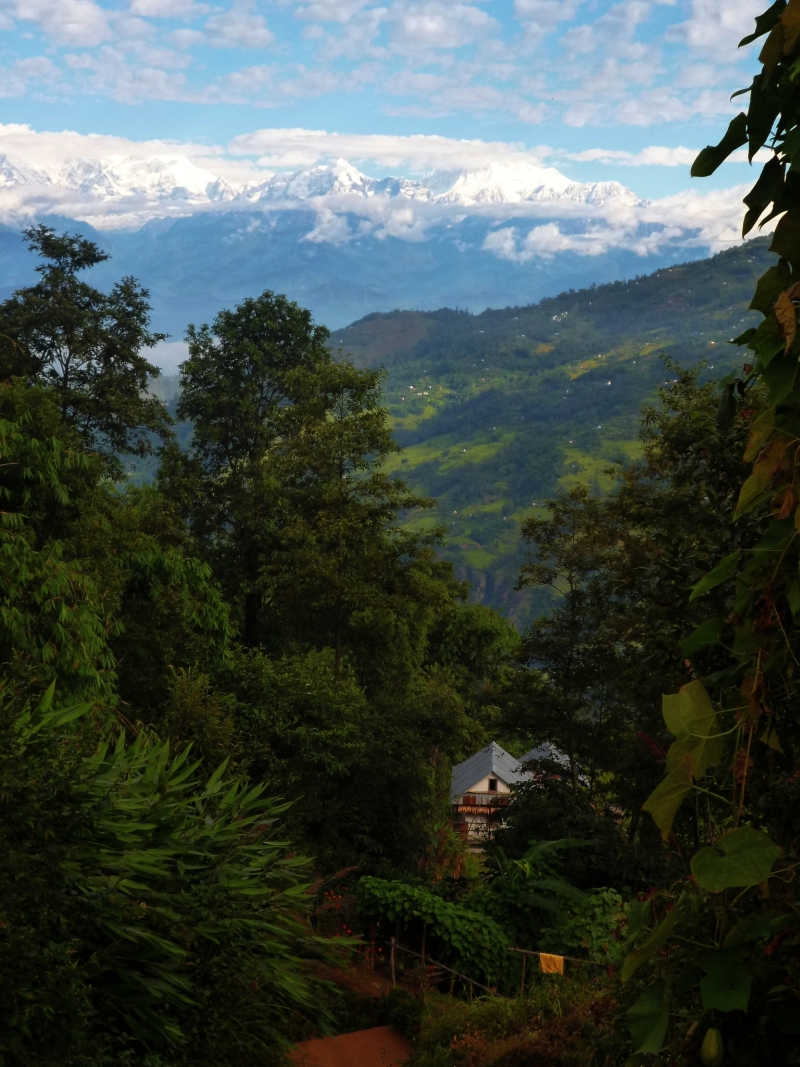
\includegraphics[width=6cm]{tumok-path.jpg}
\caption{A typical trail in Tumok}\label{tumok-path}
\end{figure}

Geomorphic deixis permeates Yakkha grammar;  it features in a number of word classes and grammatical subsystems, in demonstratives, adverbs, postpositions,  verbs and even interjections.\footnote{Other Kiranti languages like Belhare, Bantawa or Khaling furthermore distinguish altitude in their locative case systems \citep{Ebert1994The-structure, Bickel1997Spatial}.} This shows how deeply rooted the geomorphic system is in the grammar of Yakkha, and how strongly environmental factors may shape a language.\footnote{The Yakkha system (and Kiranti languages in general) also shows that spatial orientation is by no means universally egocentric (based on the body of the speaker), as had been claimed before the discovery of geomorphic deixis.} \citet{Bickeletal1999Cultural} also point out the salience of the \rede{hill} conception in cultural domains such as architecture, rituals and mythology in the Kiranti cultural sphere. For Yakkha, this connection remains to be studied.

In the following, I will briefly lay out the system, before illustrating its application in each word class. Geomorphic forms in Yakkha are based on two sets of roots, called /u/-forms and /o/-forms in the following discussion. They indicate  a threefold distinction: words based on \emph{tu} and \emph{to} for \rede{uphill}, on \emph{mu} and \emph{mo} for \rede{downhill} and on \emph{yu} and \emph{yo} for \rede{across (at the same altitude)}. The distinction between the /u/-forms and the /o/-forms is one of deictic transposition, as in Belhare (see \citealt{Bickel1997Spatial, Bickel2001Deictic}). 

The schematic diagrams in Figure \ref{deicticschema-1} and Figure \ref{deicticschema-2} provide a bird's eye view on the deictic field, and the black dots indicate the speaker. In both sets, the deictic field is partitioned into four quadrants. In the /u/-forms, the point of reference  for projecting the four quadrants (indicated by \rede{⌀}) is located within the speech situation. Objects located uphill from the interlocutors are indicated by forms based on \emph{tu}, objects located downhill  from the interlocutors are indicated by forms based on  \emph{mu}, and objects on the same level (to either side of them) are indicated by forms based on \emph{yu} (see Figure \ref{deicticschema-1}). Contrasts like left/right or front/back do exist in Yakkha, but they are rarely used in the expression of spatial orientation. The speakers are able to provide the lexemes when they are asked, but I have no instance of recorded natural speech using \emph{pheksaŋ} \rede{left} and \emph{chuptaŋ} \rede{right}. From the available lexical information, the left side is connoted negatively; it is used metaphorically in a term for a malicious wizard, for instance. This also  fits with the widespread perception of the left hand as impure in South Asian societies. The terms \emph{ondaŋ} \rede{front} and \emph{heksaŋ} \rede{back} are used more frequently than \rede{left} and \rede{right}. 


\begin{figure}
\centering
\setlength{\fboxsep}{0pt}
\fbox{
\begin{tikzpicture}[xscale=1, yscale=-1, draw=black, fill=black!30]
	\node (lo) at (-3,-3) {};
	\node (ro) at ( 3,-3) {};
	\node (lu) at (-3, 3) {};
	\node (ru) at ( 3, 3) {};
	\node (z)  at ( 0, 0) {\Large ⌀=●};
	\draw (lo)--(z);
	\draw (ro)--(z);
	\draw (lu)--(z);
	\draw (ru)--(z);
	\node (tu) at ( 0,-2) {tu};
	\node (yu1)at (-2, 0) {yu};
	\node (yu2)at ( 2, 0) {yu};
	\node (mu) at ( 0, 2) {mu};
\end{tikzpicture}
}
\caption{The deictic mapping system of the /u/-forms}\label{deicticschema-1}
\end{figure}

\bigskip

\begin{figure}
\centering
\setlength{\fboxsep}{0pt}
\fbox{
\begin{tikzpicture}[xscale=1, yscale=-1, draw=black, fill=black!30]
	\node (lo) at (-3,-3) {};
	\node (ro) at ( 3,-3) {};
	\node (lu) at (-3, 3) {};
	\node (ru) at ( 3, 3) {};
	\node (z)  at ( 0, 0) {\Large ⌀};
	\node (sp) at (-4, 0) {\Large ●};
	\path (sp.west)++(0,0) node[left]{\footnotesize(speaker)};
	\draw (lo)--(z);
	\draw (ro)--(z);
	\draw (lu)--(z);
	\draw (ru)--(z);
	\node (to) at ( 0,-2) {to};
	\node (khe)at (-2, 0) {khe};
	\node (yo) at ( 2, 0) {yo};
	\node (mo) at ( 0, 2) {mo};
\end{tikzpicture}
}
\caption{The transposed mapping system of  \emph{khe} and the /o/-forms}\label{deicticschema-2}
\end{figure}

\bigskip

\begin{figure}
\centering
\setlength{\fboxsep}{0pt}
\fbox{
\begin{tikzpicture}[xscale=1, yscale=-1, draw=black, fill=black!30]
	\node (l) at (-3, 0) {};
	\node (r) at ( 3, 0) {};
	\node (z)  at ( 0, 0) {\Large ⌀};
%	\node (sp) at ( 0, 4) {\Large ●};
% \path (sp.east)++(0,0) node[right]{\footnotesize(speaker)};
	\draw (l)--(z);
	\draw (r)--(z);
	\node (to) at ( 0,-2) {to};
	\node (mo) at ( 0, 2) {mo};
\end{tikzpicture}
}
\caption{Object-centered usage of \emph{mo} and \emph{to}}\label{deicticschema-3}
\end{figure}


In the /o/-forms, the point of reference for  projecting the four quadrants is transposed to a location that is not identical to the speech situation. The distinctions between \rede{uphill}, \rede{downhill} and \rede{across} are now determined from the perspective of this transposed point of reference (see Figure \ref{deicticschema-2}; positioning  the speaker on the left side of the diagram was an arbitrary choice, he could as well have been posited on the right side; of course with a consequent reversal of \emph{yo} and \emph{khe}). Furthermore, if the transposed zero point is on the same elevation level as the interlocutors, a fourth root \emph{khe} comes into play, indicating the field between this new zero point and the speech situation. This field opens up only in the transposed system. The transposed zero point is important for generic statements and when the speaker talks about events he saw in movies, for instance. Given the transposed zero-point, it is only natural that there are more adverbs derived from the /o/-forms than from the /u/-forms. The  /o/-forms also serve as bases for spatial postpositions. Postpositions derived from the /u-/forms would only have the potential to locate objects with respect to the speech situation, not with respect to other objects.

The /o/-forms are also used to locate objects, or parts of objects, in relation to one another, for instance in order to determine the upper and the lower floor of a house, or in statements like \rede{I climbed up the tree}, where one abstracts away from the topography. In this object-centered system of spatial orientation, the location of the speech situation is irrelevant.  This is outlined in Figure \ref{deicticschema-3}.  There are some fixed expressions like \emph{mokhaʔla-tokhaʔla} \rede{up and down} (lit.: \rede{down and up}). Similarly, \emph{yo} and \emph{khe} are used to convey contrasting directions on the same level (regardless of where the speaker is located), for instance in expressions like \emph{yokhaʔla-khekhaʔla} \rede{to and fro, back and forth}.

After this rather abstract characterization of the geomorphic orientation system of Yakkha, the remaining sections will illustrate how it is applied in each grammatical subsystem. Demonstratives (together with the interjections), are discussed in §\ref{dem-pron-2}, adverbs in  §\ref{geodeixis}, postpositions  in §\ref{geomorph-postp} and verbs in §\ref{geomorph-verb}.



\section{Demonstratives}\label{dem-pron-2}	

There are two sets of demonstratives, one featuring the the deictic /u/-forms and one featuring the transposed /o/-forms, as summarized in Tables \ref{mutuyu} and \ref{motoyo}. Structurally, these subsets are different from each other, too.  The /o/-forms are inherently adverbial and become nominal through nominalization with \emph{=na} ({\sc sg}) or \emph{=ha \ti =ya} ({\sc nsg/nc}). This is illustrated for \emph{to} in example \Next. These demonstratives can be used adnominally or pronominally. 
The /u/-forms are  essentially adverbs, too, but they can also be used as interjections, i.e. as proforms for clauses (see example \NNext). In this function they have a characteristic intonation. Uttered to attract the hearer's attention and to make him look in a particular direction, they are often accompanied by pointing gestures. The /u/-forms always locate an object with respect to the speech situation, i.e., the zero point is identical to the utterance context. This explains why the /u/-forms can combine with the proximal demonstratives, \emph{na} and \emph{kha} (cf. §\ref{dem-pron}),  to yield the topography-specific demonstratives shown in Table \ref{mutuyu}. 

\begin{table}[htp]
\begin{centering}
\begin{tabular}{lll}
\toprule
 {\sc direction} & {\sc root} & {\sc demonstrative}  \\
  & {\sc   ({\sc adv/interj})} & ({\sc sg/nsg, nc})\\
\midrule
{\sc up}&\emph{tu} &\emph{tunna/tukha}\\
{\sc across } &\emph{yu} &\emph{yunna/yukha}\\
{\sc down}&\emph{mu} &\emph{munna/mukha}\\
\bottomrule
\end{tabular}\\
\caption{Geomorphic demonstratives,  /u/-forms} \label{mutuyu}
\end{centering}
\end{table}


\begin{table}[htp]
\begin{centering}
\begin{tabular}{lll}
\toprule
 {\sc direction} & {\sc root } & {\sc demonstrative} \\
  &(adv.) & ({\sc sg/nsg, nc})\\
\midrule
{\sc up}&\emph{to} &\emph{tona/toha} \\
{\sc across (beyond)}&\emph{yo} &\emph{yona/yoha} \\
{\sc across }&\emph{khe}&\emph{khena/kheha} \\
{\sc down}&\emph{mo} &\emph{mona/moha} \\
\bottomrule
\end{tabular}\\
\caption{Geomorphic demonstratives,  /o/-forms and  \emph{khe} }\label{motoyo}
\end{centering}
\end{table}


\ex. \ag. to khy-a!\\
uphill go{\sc -imp}\\
\rede{Go up!}
\bg. to=na paŋ\\
uphill{\sc =nmlz.sg} house\\
\rede{the upper house}


\ex.\ag.muǃ puchak!\\
{\sc int} snake\\
\rede{Look, down thereǃ A snakeǃ} 
\bg.tuǃ maŋmeǃ\\
{\sc int} eagle\\
\rede{Look, up thereǃ An eagleǃ} 


Examples of /u/-demonstratives are shown in \Next.  In \Next[a], the home of the person referred to by \emph{buddhini} is located on the same level as the speaker's home, where she is sitting at the time of speaking. Example \Next[b] is from a mythical story that takes place in the environment and the array of villages as they are today, and the place called Manglabare is uphill from the speech situation (in Tumok village). The /u/-forms are also used for microlocation, such as pointing out a spider to the downhill side of the speaker, even if it is located on the same elevation level (see Figure  \ref{deixill-1}).

\ex.\ag.nhaŋ    yunna              buddhini=ca        eko pi-ŋ\\
and\_then this\_across buddhist\_woman{\sc =add} one give{\sc [pst]-1sg.A}\\
\rede{And I gave one to the buddhist woman (living) over there.}\source{36\_cvs\_06.387}
\bg.ŋ-ikt-uks-u-ci=hoŋ   tunna    maŋlabare n-da-ya-by-a-ma	\\
{\sc 3pl.A-}chase{\sc -prf-3.P[pst]-3nsg.P=seq} this\_uphill Manglabare {\sc 3pl-}come{\sc -pst-V2.give-pst-prf}\\
\rede{As they (the Limbus) chased them (Lalubang and Phalubang), they  (the Limbus) already came up to Manglabare.} (lit. \rede{to Manglabare uphill}) \source{22\_nrr\_05.029}	



\begin{figure}
\centering
\setlength{\fboxsep}{0pt}
\fbox{
	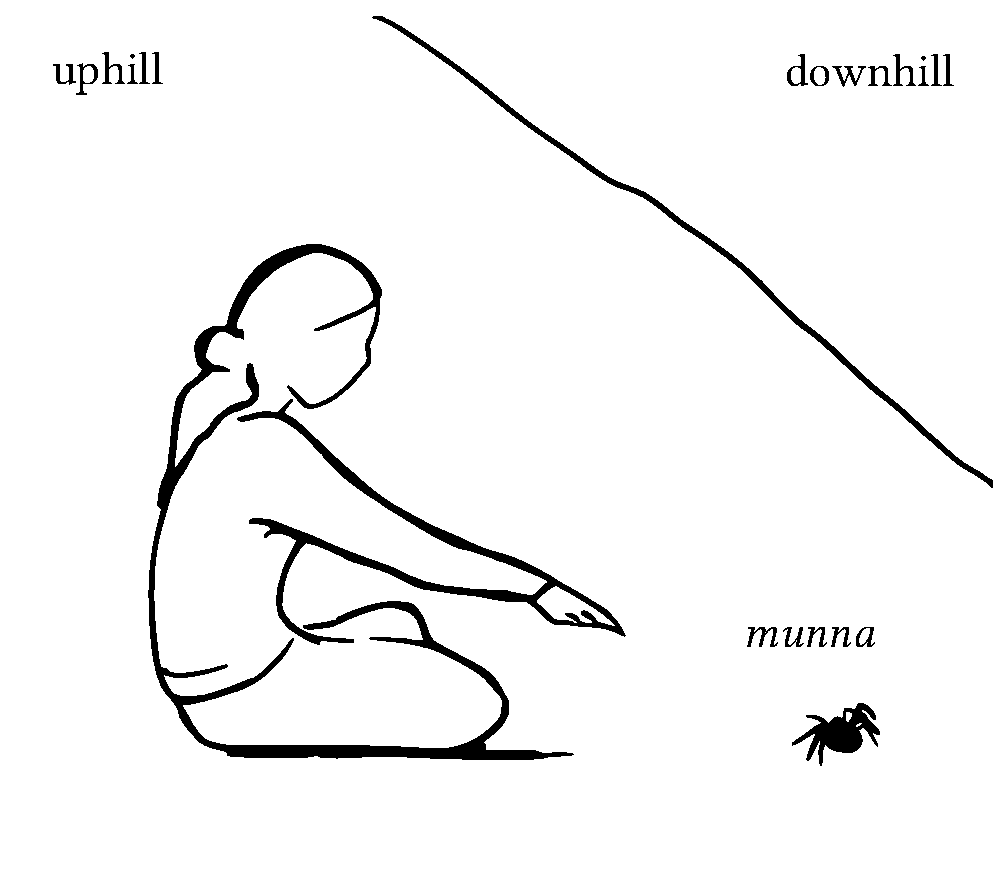
\includegraphics[width=7cm]{deixill-1.eps}
}
\caption{The /u/-forms in practice}\label{deixill-1}
\end{figure}


	
	
In contrast, the /o/-forms are found in generic statements (see \Next[a]), and in procedural descriptions, that are detached from the here and now of the speech situation (see \Next[c]). They are also found in contexts that open up a secondary deictic field, such as in movies (see example  \Next[b] from a pear story). 

\ex.\ag.\label{mewamhabu}nhaŋ eko=bu,    mo=na tala=ca         me-wa-m=ha=bu\\
and\_then one{\sc =rep} downhill{\sc =nmlz.sg} floor{\sc =add} {\sc neg-}live{\sc -inf[deont]=nmlz.nsg=rep} \\
\rede{And one more thing: the Linkhas shall not live on the ground floor, too, it is said.} \source{11\_nrr\_01.040}
\bg. nhaŋŋa hon=na mamu=nuŋ, saikal=be ta-yatasa=na yo=na mamu=ca, nhaŋŋa khaʔla lukt-a-sy-a-ci,  men=na=i?	\\
	and\_then that\_very{\sc =nmlz.sg} girl{\sc =com} bicycle{\sc =loc} come{\sc [3sg]-pst.prog=nmlz.sg} across{\sc =nmlz.sg} girl{\sc =add} and\_then like\_this bump\_into{\sc -pst-mddl-pst-du} {\sc cop.neg=nmlz.sg=q}\\
\rede{And that earlier girl and the girl that was coming on the bike, they collided like this, right?}\footnote{The verb form \emph{tayatasa} could not be analyzed, as no corresponding paradigm could be elicited. According to the Nepali translations, I tentatively labelled it \rede{past progressive}.} \source{34\_pea\_04.025 }
\bg.to=na  paŋ=be     ku-nuŋ-ma, sin-di-me,  mo=na  paŋ=be     tha  n-leŋ-me-n, ka-ma pʌryo  ai?\\
up{\sc =nmlz.sg} house{\sc =loc} guard{\sc -V2.sit-inf[deont]} die{\sc -V2.give[3sg]-npst} downhill{\sc =nmlz.sg} house{\sc =loc} knowledge {\sc neg-}happen{\sc [3sg]-npst-neg}, say{\sc -inf[deont]} have\_to {\sc tag}\\
\rede{In the upper house, people keep sitting at the sickbed, someone dies eventually ‒ in the lower house, they have no idea, one has to tell them, right?}\footnote{This example refers to another Yakkha custom: firing rifles for announcements, in pairs to announce marriages, and in single shots to announce the death of a  member of the household. The choice of \emph{tona} and \emph{mona} in this example is arbitrary, it could as well be the other way round, as this is just an example made by the speaker to illustrate the custom; the sentence does not refer to any particular constellation of houses.} 	 \source{29\_cvs\_05.028}
   			
			
As pointed out in the introduction, the /o/-forms are also used when two objects are located with respect to each other, as in such cases the zero point is also not identical to the speech situation, but located between the related objects, such as in \Next. In this example, two people look downhill, seeing two swallows  sitting on a parallel wires (as illustrated in Figure \ref{deixill-2}). Interlocutor A points out something about one of the  swallows and interlocutor B wants to reconfirm whether he got the reference right. The  zero point for the projection is located between the two birds. The demonstrative \emph{tona} refers to the bird closer to the hill on which the interlocutors are located and that serves as the anchor of the relation, and \emph{mona} refers to the bird on the wire  further away from that hill. If the swallows had been located uphill from the interlocutors, the question would have been exactly the same as the one uttered in \Next; the speech situation is irrelevant for the interpretation of this utterance.

\exg.\label{ex-gumthali}to=na=em mo=na=em?\\
uphill{\sc =nmlz.sg=alt} downhill{\sc =nmlz.sg=alt}\\
\rede{(Do you mean) the upper one or the lower one?}

\begin{figure}
\centering
\setlength{\fboxsep}{0pt}
\fbox{
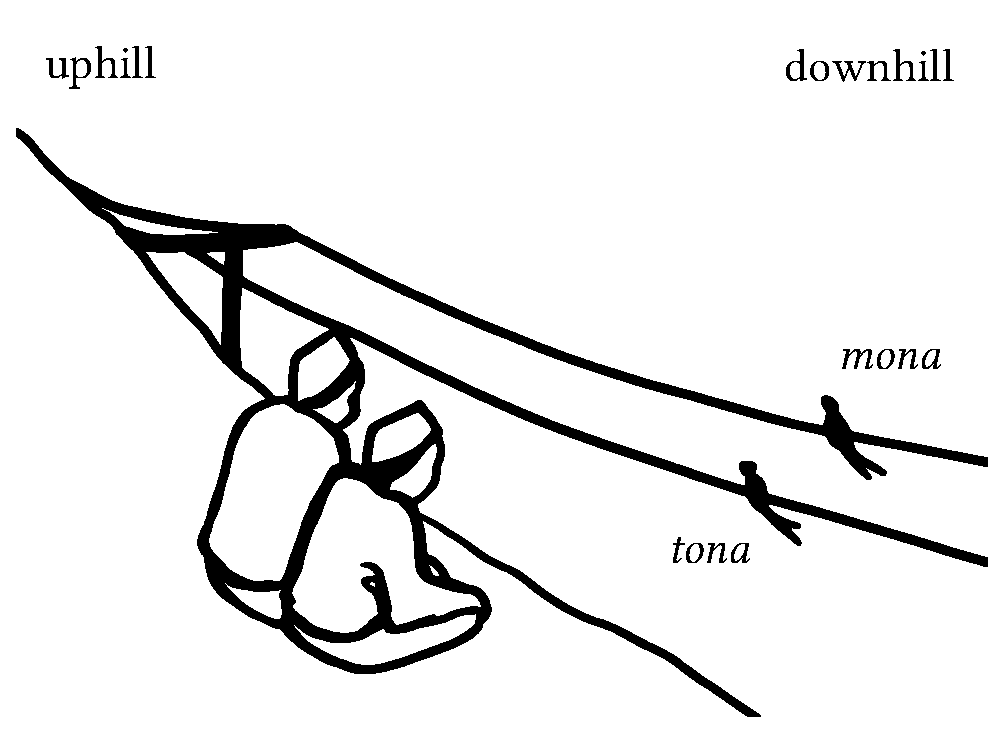
\includegraphics[width=7cm]{deixill-2.eps}
}
\caption{Illustration for example \ref{ex-gumthali}}\label{deixill-2}
\end{figure}

The uphill-downhill distinction can also be mapped onto the human body, as in \Next. These designations are used regardless of the orientation of a person, thus instantiating an exception to the topography-based system.

\ex.\ag.mo=ha keŋ=ci \\
downhill{\sc =nmlz.nsg} tooth{\sc =nsg} \\
\rede{lower teeth}
\bg.to=ha keŋ=ci\\
uphill{\sc =nmlz.nsg} tooth{\sc =nsg} \\
\rede{upper teeth} 


Things look slightly different on the horizontal plane: in example \Next[a], two houses are identified  that are both on the same altitude level as the interlocutors. The house further away is referred to as \emph{yona}, the closer one is \emph{khena}, a distinction most closely rendered by \rede{there, thither} and \rede{here, hither} in the English translation (see also Figure \ref{deixill-3}, which  features  \emph{mo} and \emph{to} as well). In Figure \ref{deixill-3}, the couple in the foreground represents the speech situation.

\ex.\ag.\label{khenamenna}eh, khe=na paŋ menna, yo=na=le\\
oh across\_here{\sc =nmlz.sg} house {\sc neg.cop=nmlz.sg} across\_there{\sc =nmlz.sg=ctr}\\
\rede{Oh, not the closer house, the next oneǃ} 
 \bg. mela=be      yo   khe    son-ca-saŋ\\
market{\sc =loc} across\_there across\_here look{\sc -V2.eat-sim} \\
\rede{Looking around in the market, ...} \source{01\_leg\_07.152}
 
\begin{figure}
\centering
\setlength{\fboxsep}{0pt}
\fbox{
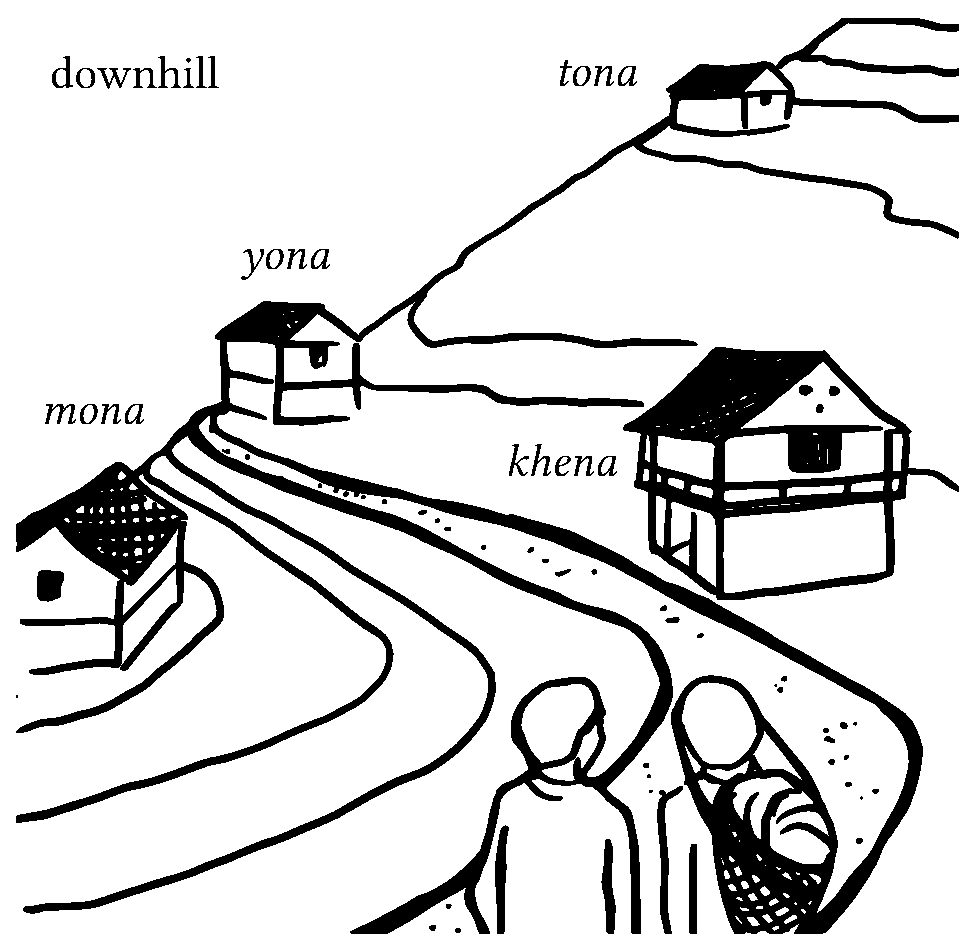
\includegraphics[width=7cm]{deixill-3.eps}
}
\caption{The transposed system in practice}\label{deixill-3}
\end{figure}

The quadrant indicated by \emph{yo} is always beyond some (real or imagined) boundary on the horizontal level, i.e. it is projected from a zero point that must be distinct from the speech situation. The space between that boundary and the speech situation is the field indicated by \emph{khe}.\footnote{In this light, it also makes sense that \emph{khe} is never used in opposition to \emph{yu}. A \emph{khe}-quadrant opens up only when the zero point for the projection is transposed, while the field indicated by \emph{yu} projects directly from the speech situation.} In  example \Last[a], the  utterance context is relevant for the interpretation of \emph{yo} and \emph{khe},\footnote{Note that it is not the case that \emph{yona} always refers to the object between an upper and a lower object (the same is true for Belhare, see \citet{Bickel2001Deictic}).  If the speakers were standing on the level of the lower house, the demonstrative referring to it would change from \emph{mona} to \emph{yona}.} while this is not the case for the \emph{mo/to} distinction in \LLast[b], for instance. As mentioned above, the \emph{yo}/\emph{khe}  contrast can also be used generically, independent  of any particular utterance context, as in example  \Last[b].
 
As the /u/-forms always rely on information that is retrievable from the utterance context, they are not compatible with the reportative marker \emph{=bu}. Thus, while \Next[a] is perfectly fine, \Next[b] is pragmatically awkward.\footnote{The reportative marker can also be found on embedded speech, both direct and indirect; see also §\ref{utterance-pred} and §\ref{hearsay}.} Another example for /o/-forms combining with \emph{=bu} is \ref{mewamhabu} above.

\ex.\ag. to=na minuma lukt-a-khy-a=na=bu?\\
uphill{\sc =nmlz.sg} cat run{\sc [3sg]-pst-V2.go-pst=nmlz.sg=rep} \\
\rede{It was said that the upper cat ran away?}
\bg.?tu-nna minuma lukt-a-khy-a=na=bu?\\
this\_uphill cat run{\sc [3sg]-pst-V2.go-pst=nmlz.sg=rep} \\
Intended: \rede{It was said that the cat up there ran away?}
 
The examples in \Next show that the proximal/distal demonstratives (see  §\ref{dem-pron-1}) and the \rede{uphill}/\rede{downhill} demonstratives are not mutually exclusive; they can be used together in one syntagm. The former indicate proximity or distance to the speaker, while the latter locate the objects with respect to each other and the cline of the hill. In \Next[a], the zero point is located between the upper and the lower rocks of a group of rocks, and in \Next[b], the zero point is located in the middle of the road.\footnote{As the proximal/distal demonstratives \emph{na/nna} show a functional overlap with \emph{khena} and \emph{yona}, these two sets are not expected to occur together.}

\ex.\ag.  na   mo=na  luŋkhwak\\
this downhill{\sc =nmlz.sg} stone\\
\rede{this lower rock (of a group of rocks)} \source{37\_nrr\_07.031}
\bg.mo=na  u-lap,          to=na  u-lap,          na   lambu ghak ak=ka=i!\\
downhill{\sc =nmlz.sg} {\sc 3sg.poss-}wing uphill{\sc =nmlz.sg}  {\sc 3sg.poss-}wing this road all {\sc 1sg.poss=gen=emph} \\
\rede{The uphill side, the downhill side, this road is all mine!}  \source{36\_cvs\_06.206}


The examples in \Next illustrate abstractions away from the closest hill as the achoring element. In \Next[a],  \emph{mu} refers to a place outside the hills and far away (Germany). In \Next[b], via reduplication of the initial CV-cluster, the root  intensifies its meaning, i.e. \emph{tutunna} refers to an object further away than \emph{tunna}. These reduplications are also found in the corresponding adverbs (see §\ref{geodeixis} below). 

\ex. \ag. mu, [...] nniŋ=ghe i=ha cog-wa-m-g=ha?\\
	downhill [...] {\sc 2pl.poss=loc} what{\sc =nmlz.nsg} do{\sc -npst-2pl.A-2=nmlz.nsg}\\
	\rede{Downhill, where you live, what do you do (when someone dies)?} \source{29\_cvs\_05.008}
\bg. tunna cokcoki=nuŋ tu-tunna cokcoki\\
		that\_uphill star{\sc =com}	{\sc redup-}that\_uphill star\\
	\rede{the star up there and the star even further up}


\section{Adverbs}\label{geodeixis}

This section discusses the adverbs that belong to the geomorphic  orientation system. In §\ref{dem-pron} a set of adverbs has been introduced that is based on a proximal/distal/anaphoric distinction. The adverbs discussed in the following are based on the same distinctions between /o/-forms and /u/-forms as the demonstratives discussed in §\ref{dem-pron-2} above. 
Tables \ref{deic-all1} and \ref{deic-all2}  provide an overview of all geomorphic adverbial expressions in Yakkha. 
	 	  
 \begin{table}[htp]
\begin{centering}
\begin{tabular}{llll}
\toprule
									&{\sc up}		&{\sc across}&{\sc down}\\
\midrule
			{\sc loc/interj}	&\emph{tu}&\emph{yu}&\emph{mu}\\
			{\sc loc-prox}&\emph{tunhe}&\emph{yunhe}&\emph{munhe}\\
			{\sc loc-dist}&\emph{tunnhe}&\emph{yunnhe}&\emph{munnhe}\\
			{\sc loc-dist-emph}&\emph{tutunnhe}&\emph{yuyunnhe}&\emph{mumunnhe}\\
\bottomrule
\end{tabular} 
\caption{Geomorphic adverbs, the /u/-forms}\label{deic-all1}
\end{centering}
\end{table}

 \begin{table}[htp]
\begin{centering}
\begin{tabular}{lllll}
\toprule
									&{\sc up}		&\multicolumn{2}{l}{{\sc across}}&{\sc down}\\
											&				&{\sc prox}&{\sc dist}&\\
\midrule 	  
			{\sc loc/dir}	&\emph{to}&\emph{khe}&\emph{yo}&\emph{mo}\\
			{\sc dir} 				&\emph{tokhaʔla}&\emph{khekhaʔla}&\emph{yokhaʔla}&\emph{mokhaʔla}\\
			{\sc abl/dir}											&\emph{tondaŋ}&\emph{khendaŋ}&\emph{yondaŋ}&\emph{mondaŋ}\\
			{\sc level}											&\emph{topparik}&\emph{khepparik}&\emph{yopparik}&\emph{mopparik}\\
			{\sc level-abl}									&\emph{topparindaŋ}&\emph{khepparindaŋ}&\emph{yopparindaŋ}&\emph{mopparindaŋ}\\
			{\sc quant} 					&\emph{torok}&\emph{kherek}&\emph{yorok}&\emph{morok}\\
			{\sc quant-emph}								&\emph{toʔtorok}&\emph{kheʔkherek}&\emph{yoʔyorok}&\emph{moʔmorok}\\
			{\sc loc-prox}									&\emph{naʔto}&\emph{naʔkhe}&\emph{naʔyo}&\emph{naʔmo}\\
			{\sc loc-dist}										&\emph{nnaʔto}&\emph{nnaʔkhe}&\emph{nnaʔyo}&\emph{nnaʔmo}\\
			{\sc loc-prox-quant}					&\emph{naʔtorok}&\emph{naʔkherek}&\emph{naʔyorok}&\emph{naʔmorok}\\
\bottomrule
\end{tabular} 
\caption{Geomorphic adverbs, /o/-forms and \emph{khe}}\label{deic-all2}
\end{centering}
\end{table}


The adverbs based on the proximal/distal distinction are \emph{nhe} \rede{here} (see \Next[a]) and \emph{nnhe} \rede{there} (with initial gemination of the nasal). The adverb \emph{nnhe} is used to refer to distant locations and to locations in another deictic field, as it is opened up by a movie, for instance  (see \Next[b] from a pear story) or by talking on the phone. The anaphoric form is \emph{honnhe} \rede{just there, at a location mentioned earlier} (see also §\ref{dem-set1rel}). 

\ex. \ag. imin=na,       haku nhe, hen=se;         haku soʔ-ma=na=lai!\\
how{\sc =nmlz.sg}  now here today{\sc =restr} now look{\sc -inf[deont]=nmlz.sg=excla}\\
\rede{How is he; now he (the prospective groom) is here, only today; now we have to look at him!}  \source{36\_cvs\_06.374}
\bg.ɖhakani=be    s-wa,         nnhe  eko man=na \\
basket{\sc =loc} look{\sc -npst[3sg.P]} there one {\sc cop.neg=nmlz.sg}\\
\rede{He looks into the basket, and there is not even one.} \source{34\_pea\_04.040 }


These proximal and distal adverbs can be specified further by combining them with the /u/-forms of the geomorphic set, in the same way as it has been shown above for the demonstratives. Both sets rely on the utterance context, and are, therefore, compatible. Altogether, one arrives at three more forms for each  \rede{here} and \rede{there}: \emph{tunhe/tunnhe} \rede{up here/there}, \emph{munhe/munnhe} \rede{down here/there} and \emph{yunhe/yunnhe} \rede{across here/there}. The resulting complex forms are illustrated by the examples in \Next. 

\ex.\ag.\label{tikamunhe}ŋkha=nuŋ   nhe  gobar,   pik=ka    u-hi,    bachi=ga,        goru=ga    men=na,    munhe     khaʔla   yuŋ-ma=hoŋ      ʈika    waʔ-meʔ-ma  \\
that{\sc =com} here cow\_dung cow{\sc =gen} {\sc 3sg.poss-}shit cow{\sc =gen} ox{\sc =gen} {\sc neg.cop=nmlz.sg} down\_here like\_this put{\sc -inf=seq} blessing wear{\sc -caus-inf[deont]}\\
\rede{With this (\emph{dubo} grass), here, cow dung, from a female cow, not from an ox, one has to place it down here like this and apply a blessing (at the main door of the house).} \source{31\_mat\_01.089}
\bg.munnhe     sombare  daju=ge            ŋ-waʔ=ya=ci=bu,                      hau   jeppa!\\
down\_there Sombare eB{\sc =loc} {\sc 3pl-}exist{\sc =nmlz.nsg=nsg=rep} {\sc excla} really\\
\rede{Oh! Sombare brother down below has some (mushrooms), they say, really!} \source{13\_cvs\_02.079}
\bg. ka=go      tunnhe   bhitta=be    heʔ-ma-sy-a-ŋ=na=le,   a-na=ŋa,     uks-a-ga=i,       uks-a ly-a-ŋ=hoŋ\\
{\sc 1sg=top} up\_there wall{\sc =loc} cut{\sc -inf-aux.prog-pst-1sg=nmlz.sg=ctr} {\sc 1sg.poss-}eZ{\sc =erg} come\_down{\sc -imp-2=emph} come\_down{\sc -imp} tell{\sc -pst-1sg=seq}\\
\rede{I was cutting (grass) up there at the wall, but my elder sister said: please come down, come down, ...} \source{28\_cvs\_04.315}

As example \Next shows, the /u/-forms can also be used independently, in adverbial function. 

\exg.mu     jeʈha=ŋa   biha     cog-a             bhoŋ, mu     jeʈha=ŋa            hiŋ-ma=na\\
down first\_born\_male{\sc =erg} marriage do{\sc [3sg]-sbjv} {\sc cond} down first\_born\_male{\sc =erg} support{\sc -inf[deont]=nmlz.sg}\\
\rede{If Jetha down here marries a girl, he has to care for her.} (pointing to someone sitting in the same room as the speaker, but in the corner pointing downhill) \source{28\_cvs\_04.127}


A natural example of a reduplicated form is shown in \Next. Typically, the reduplicated forms contrast an object further away with a closer object. In this example, however, the emphasis usually connected to this reduplication is not very strong;  in the afterthought at  the end of the sentence, the simple form \emph{tunnhe} is used.\footnote{The mirative (see §\ref{ptcl-evid})  is used here because the speaker finally remembers where she had been at a particular day some weeks prior to this conversation.} For instance, if the speaker points downhill towards two houses, the closer location is indicated by \emph{munnhe} \rede{down there} and the one further down is indicated by \emph{mumunnhe} \rede{further down there}. 

	\exg. ka  ŋkhaʔla bhoŋ tu-tunnhe         bhauju=ghe               wa-ya-masa-ŋ=na                        raecha, tunnhe=ba\\
	{\sc 1sg} like\_that {\sc cond} {\sc redup}-there\_uphill sister-in-law{\sc =loc} be{\sc -pst-pst.prf-1sg=nmlz.sg} {\sc mir} there\_uphill{\sc =emph}\\
\rede{If it is like that, I had been uphill at my sister-in-law's house, just up there.} \source{36\_cvs\_06.399}


The /o/-forms are used when the zero point is not located within the speech situation. Thus, they cannot combine in one word with the deictic forms \emph{nhe} and \emph{nnhe}. They can combine with other morphology, e.g. with case markers, to convey a variety of spatial notions, such as ablative and directive, shown in \Next. The roots \emph{mo}, \emph{to} and \emph{yo} are inherently locative, so that they cannot combine with the locative \emph{=pe} (for instance, *\emph{mobe} is ungrammatical). Forms as in \Next[a] can be used both with an ablative and a directive reading.

\ex. \ag.mondaŋ ky-a=na.\\
from\_below come\_up{\sc [3sg]-pst=nmlz.sg}\\
\rede{He came up from below.}
\bg. yondaŋ    eko mamu a-cya            we=ppa=ʔlo!\\
from\_over\_there one girl {\sc 1sg-}child exist{\sc [3sg;npst]=emph=excla}\\
\rede{(But) I have a daughter from (my ex-husband) over there!} \source{06\_cvs\_01.018}
\bg.tokhaʔla khy-aǃ\\
upwards go{\sc -imp}\\
\rede{Go upwardsǃ}

The contrast between \emph{yo} and \emph{khe} (see also Figure \ref{deicticschema-2} above) can be illustrated by the following context: the two villages Madi Rambeni and Madi Mulkharka are both located on a hill next to the hill on which Tumok is situated (see also the Map in Figure \ref{map-sank} in §\ref{geogr}). These two hills are separated by a river (the Maya Khola), and thus both Madi Rambeni and Madi Mulkharka qualify as \emph{yo} \rede{across} from Tumok. Both villages are roughly on the same altitude level as Tumok, but while Madi Mulkharka is right across (one can see its houses), Madi Rambeni is further away and out of sight. Thus, in a conversation (in Tumok) contrasting the two villages, Madi Mulkharka would be indicated by \emph{khe}, while Madi Rambeni would be referred to by \emph{yo}, since it is further away from Tumok  than Madi Mulkharka.

Another set of adverbs is instantiated by adverbs such as \emph{mopparik} \rede{right below} in \Next. It refers to a place that is right below the point of reference, like a lower floor or a lower step on a ladder (\emph{-parik} comes from the Nepali noun \emph{paṭī} \rede{side}).\footnote{The change of  coronal plosives to rhotics in intervocalic position is also attested elsewhere in the language, and closing a word-final CV syllable with /k/ is a common process in the \rede{Yakkhafication} of lexical material from Nepali, see §\ref{loansphon}.} This set of adverbs, like the forms in \Last, can also be used  as  postpositions (see §\ref{geomorph-postp} below). 

\exg. honna              sem-khuba        babu, pheri, i=ʔlo       mopparik    jhar-a          cok-ma-sy-a=na\\
that\_very pluck{\sc -nmlz} boy again what{\sc =excla} right\_below descend{\sc -nativ} do{\sc -inf-aux.prog-pst[3sg]=nmlz.sg} \\
\rede{That guy who was plucking, he was climbing down (the ladder).} \source{34\_pea\_04.036}


Furthermore, there are forms ending in the syllable \emph{-rok \ti -rek}, i.e. \emph{morok}, \emph{torok}, \emph{yorok} and \emph{kherek}. They convey that something is located (or moving) a bit more in the respective direction than had been presupposed, thus quantifying the distance (see \Next). Example \NNext illustrates the same with ablative forms. 

\ex. \ag.hoŋkhaʔniŋŋa   naʔmasek    khi-khuwa          yapmi=ci     yorok      torok      ŋ-wa-ya-masa\\
that\_very\_time night fight{\sc -nmlz} person{\sc =nsg} a\_bit\_further a\_bit\_up {\sc 3pl-}be{\sc -pst-pst.prf}\\
\rede{At that time, those fighting people had been (scattered) a bit further away and a bit further uphill.} \source{41\_leg\_09.057}
\bg.nna  ten=be=jhen,         mo,   yondaŋ    morok=ŋa       limbu=ci=ca           ŋ-wa-ya-ma\\
that village{\sc =loc=top} down from\_across a\_bit\_down{\sc =ins} Limbu\_person{\sc =nsg=add} {\sc 3pl-}be{\sc -pst-prf}\\
\rede{In that village below, across and then a bit below from there, Limbu people were  living, too.} \source{22\_nrr\_05.009}

\ex. \ag.mondaŋ kham ket-u-eba\\
from\_below ground bring\_up{\sc -3.P[imp]-pol.imp}\\
\rede{Bring up mud from below.}
\bg.miyaŋ morondaŋ ket-u-eba\\
a\_little from\_further\_below bring\_up{\sc -3.P[imp]-pol.imp}\\
\rede{Bring it up from a bit further below.} (Context: the mud is better further downhill.)

The adverbs ending in \emph{-rok\ti -rek} can also be partly reduplicated, yielding forms like \emph{moʔmorok} or \emph{toʔtorok}. Tentatively, in analogy to the reduplications discussed above, I conclude that this amplifies the distance, too, but there are not enough examples in my data for any strong claims. The reduplicated forms are also  used when nothing has been presupposed (cf. also §\ref{geomorph-postp} on postpositions).
 
\exg.  beuli siŋgara         cok-se         miyaŋ yoʔyorok ŋ-ghet-wa\\
bride a\_wedding\_custom do{\sc -sup} a\_little a\_bit\_further {\sc 3pl.A-}take{\sc -npst[3.P]}\\
\rede{To dress the bride with the sari that the groom got her, they take her a bit further away.} \source{25\_tra\_01.043}


The last set of adverbs introduced here has  the forms \emph{naʔmo}, \emph{nnaʔmo}, \emph{naʔyo}, and so on. They are composed of the singular forms of the proximal/distal demonstratives and the /o/-forms, conveying \rede{down here}, \rede{down there}, \rede{across here} and so on (see Table \ref{deic-all2}).  The cognate forms in Belhare are demonstratives that are marked for environmental case (see \citealt[226-27]{Bickel2001Deictic}). The environmental case system was probably present in earlier stages of Yakkha, too, but apart from these adverbial forms, there is no trace of such a system synchronically. The forms have characteristic stress, i.e. on the first syllable. They locate the utterance context from the perspective of another location. In \Next[a], the zero point is Manglabare, a place above Tumok (the place of speaking, referred to by \emph{naʔmo} \rede{down here}). In \Next[b], the point of reference is the sky, mentioned in the adverbial clause.  The sentence in \Next[c] was uttered by someone who confused two roads, and the point of reference is the point of departure of the speaker's movement, before she confused the roads.

\ex. \ag.haku nnakha lalubaŋ=nuŋ   phalubaŋ=ga    ten=go         naʔmo=maŋ      sa,     eŋ=ga=e\\
now those Lalubang{\sc =com} Phalubang{\sc =gen} village{\sc =top} down\_here{\sc =emph} {\sc cop.pst[3sg]} {\sc 1pl.incl.poss=gen=loc}\\
\rede{Now, that village of Lalubang and Phalubang, though, was down  here, in our area.} \source{22\_nrr\_05.034}
\bg. na   taŋkheŋ=be    pes-a-khy-a-ma=niŋa naʔmo heko=ha nwak=ci=ŋa haku nda nhe uŋ-ma n-dokt-wa-ga-n=na n-lu-ks-u\\
	this sky{\sc =loc} fly{\sc -pst-V2.go-pst-prf[3sg]=ctmp} down\_here other{\sc =nmlz.nsg} bird{\sc =nsg=erg}	now {\sc 2sg} here come\_down{\sc -inf} {\sc neg-}get\_to\_do{\sc -npst-2.A[3.P]-neg=nmlz.sg} 	{\sc 3pl.A}-tell-{\sc prf-3.P[pst]}\\
	\rede{When he flew up into the sky, down here the other birds told him: Now you will not get the chance to come down here any more.} \source{21\_nrr\_04.034-5}
\bg.	naʔyo=le             sa-ŋ=na,                 nnaʔyo=le             khy-a-ŋ=na?\\
over\_here{\sc =ctr} {\sc cop.pst-1sg=nmlz.sg} over\_there{\sc =ctr} go{\sc -pst-1sg=nmlz.sg}\\
\rede{But I was over here, did I go over there?} \source{28\_nrr\_04.030}


With the introduction of these forms, one arrives at two sets that are translatable as \rede{down/up/across here} and \rede{down/up/across there}, for instance \emph{naʔmo}  and forms like  \emph{munhe} for \rede{down here}. The  contrast between forms like  \emph{naʔmo}  and  \emph{munhe} is, of course, the zero point. While \emph{naʔmo} implies a perspective from a location outside the speech situation (see \Last and \Next), \emph{munhe} refers to a location in the downhill quadrant, as projected from the perspective of the speaker (see e.g. examples \ref{tikamunhe}—(c) above).  The speaker can choose whether he wants to locate objects from his own perspective or from someone else's perspective, and sometimes this is fixed by sociolinguistic conventions. In imperatives, for instance, it would be inappropriate to use one's own perspective, they are always expressed with /o/-forms, as in \Next. 

\ex. \ag.naʔyo ab-a\\
over\_here come\_across{\sc -imp}\\
\rede{Come over here (from where you are).}
\bg.naʔmo uks-a\\
down\_here come\_down{\sc -imp}\\
\rede{Come down here (from where you are).}


The \rede{quantifying} or \rede{degree} derivation via \emph{-rok} that was introduced above is also possible with \emph{naʔto} (and the related forms), yielding forms like \emph{naʔtorok} \rede{a bit closer up here}.



\section{Postpositions}\label{geomorph-postp}

The geomorphic postpositions are formally identical to the adverbs described in §\ref{geodeixis}. They take nominal complements that are marked by the genitive case (see §\ref{case-gen}). The possessive prefix is, however, not possible on these postpositions, which distinguishes  them from relational nouns (cf. §\ref{postpos-2}). Table \ref{relnoun-topo} provides an overview on the postpositions.

 \begin{table}[htp]
\begin{centering}
\begin{tabular}{lll}
\toprule
{\sc postposition}&{\sc gloss}&{\sc internal structure}\\
\midrule
\emph{mopparik} &right below&\rede{downhill-side[Nep.]}\\
\emph{topparik} &right above&\rede{uphill-side[Nep.]}\\
\emph{yopparik} &right across&\rede{across-side[Nep.]}\\
\emph{mokhaʔla} &below, downwards&\rede{uphill-{\sc dir}}\\
\emph{tokhaʔla} &above, upwards&\rede{uphill-{\sc dir}}\\
\emph{yokhaʔla} &across, away&\rede{across-{\sc dir}}\\
\emph{mondaŋ} &from below&\rede{downhill-{\sc abl}}\\
\emph{tondaŋ} &from above&\rede{uphill-{\sc abl}}\\
\emph{yondaŋ} &from the same level&\rede{across-{\sc abl}}\\
\emph{moʔmorok} &a bit below&\\
\emph{toʔtorok} &a bit above&\\
\emph{yoʔyorok} &a bit further away&\\
\emph{kheʔkherek} &a bit closer&\\
\bottomrule
\end{tabular} 
\caption{Geomorphic postpositions}\label{relnoun-topo}
\end{centering}
\end{table}

The postpositions \emph{mopparik} and \emph{topparik} indicate a relation of parallel planes located above/below each other, such as stacked books or floors of a house (see \Next[a]). Example \Next[b] shows a corresponding adverbial in a (semi-transparent) ablative form.\footnote{In analogy to these examples, one could assume that  there is also a directional \emph{topparikhaʔla}/\emph{mopparikhaʔla} to indicate directedness towards an upper/lower level, but such forms do not exist. Probably, \emph{topparik} (and related forms) also have a directional meaning.}  The same is possible with \emph{yopparik} and \emph{khepparik} on the horizontal level.

If the speaker wants to express that an object  is oriented towards a particular direction, the directional forms \emph{tokhaʔla}, \emph{mokhaʔla}, \emph{yokhaʔla} and \emph{khekhaʔla}  are used; orientation away from another object is indicatd by the ablative forms  \emph{tondaŋ}, \emph{mondaŋ},   \emph{yondaŋ} and \emph{khendaŋ}  (see \NNext).
 
\ex. \ag.ʈebul=ga mopparik\\
table{\sc =gen} right\_below\\
\rede{below the table (on a lower level, e.g. on the ground)}
\bg.kanciŋ mopparindaŋ ky-a-ci=ha\\
{\sc 1du} from\_right\_below come\_up{\sc -pst-du=nmlz.nsg}\\
\rede{We came up from the lower floor.}

\ex. \ag.ʈebul=ga tokhaʔla\\
table{\sc =gen} upwards\\
\rede{above the table (e.g. a lamp installed on the wall)}
\bg. ʈebul=ga mondaŋ chwigam kept-u=na\\
table{\sc =gen} from\_below chewing\_gum  glue{\sc -3.P[pst]=nmlz.sg}\\
\rede{Someone stuck chewing gum below the table.}

The partly reduplicated forms \emph{moʔmorok, toʔtorok} and \emph{yoʔyorok} convey that an object is located a bit in the respective direction, from the perspective of the object referred to by the complement noun (see \Next).

\ex. \ag.uŋci-paŋ=ga           moʔmorok          eko hoŋma wei-sa=na\\
{\sc 3nsg.poss-}house{\sc =gen}  bit\_downhill one river exist{\sc -pst[3sg]=nmlz.sg}\\
\rede{A bit downhill from their house there was a river.} \source{01\_leg\_07.283}
\bg.hon=na         yuktham=ga    yoʔyorok     kheʔkherek\\
that\_very{\sc =nmlz.sg} place{\sc =gen} bit\_further bit\_closer\\
\rede{around that place/the surroundings of that place} \source{01\_leg\_07.269}
		
		

\section{Motion verbs}\label{geomorph-verb}

Several motion verbs have also lexicalized the uphill/downhill distinction, as shown in example \Next and in Table \ref{deic-verb}. Event specification with regard to the topography is highly frequent. Even though neutral forms are available (also included in the table), the pragmatically expected forms are those specifying the event for the \emph{mo/to/yo} distinction. This specificity reaches well beyond \rede{classical} motion events. Small-scale motions, too, like putting, repairing, stacking, looking, turning or calling are often precisely specified with respect to their spatial orientation. This is achieved by means of complex predicates  with different function verbs  (see \Next[b] and Table \ref{V2-table} in Chapter \ref{verb-verb}). Motion away from a point of reference is not specified with respect to the topography, there are only the neutral verbs \rede{go} and \rede{carry off}. This is unexpected pragmatically: in motion events towards a point of reference, the speaker and the hearer are usually identifiable, and with them, the direction of the movement. In motion events away from a point of reference, as in \rede{go} and \rede{carry off}, the direction of the movement is less predictable, and therefore, it would be  more important pragmatically to specify events of going with regard to the topography-based distinctions.
 

\begin{table}[htp]
\begin{centering}
\begin{tabular}{lll}
\toprule
 & {\sc come} &  {\sc bring}  \\
\midrule
{\sc neutral}&\emph{ta} \rede{come} (from a greater distance)& \emph{taʔ} \rede{bring}\\
{\sc neutral}&\emph{kheʔ} \rede{go} & \emph{khet} \rede{carry off}\\
{\sc up}&\emph{keʔ} \rede{come up}& \emph{ket} \rede{bring up}\\
{\sc across}&\emph{ap} \rede{come} (same level, small distance)& \emph{apt} \rede{bring}\\
{\sc down}&\emph{uks \ti uŋ} \rede{come down}&\emph{ukt} \rede{bring down} \\
\bottomrule
\end{tabular}
\caption{Geomorphic distinctions in motion verbs}\label{deic-verb}
\end{centering}
\end{table}


\ex. \ag.kanciŋ  to  tub-i=hoŋ          uks-a-ŋ-ci-ŋ=hoŋ                       yo      tas-a-ŋ-c-u-ŋ=ba\\
{\sc 1pl} up meet{\sc -1pl=seq} come\_down{\sc -pst-excl-du-excl=seq} across arrive{\sc -pst-excl-du-3.P-excl=emph}\\
\rede{Having met  uphill (many people), we (two) came down (home) and arrived across (at a neighbour's house on the same level as the speaker's home).} \source{36\_cvs\_06.395}
\bg.na   eko=ŋa=go       thend-u-get-uks-a=ba,     nna, om     leks-a=niŋa\\
this one{\sc =erg=top} lift{\sc -3.P-V2.bring\_up-3.P-prf-pst=emph} that bright become{\sc -pst[3sg]=ctmp}\\
\rede{One of them lifted it (the rock) and carried it up (holding in his hands, not carrying on his back), while the sun came out.} \source{37\_nrr\_07.086}


These topography-specific verbs are only compatible with suitable adverbial expressions. For instance, \emph{apma} \rede{come over} can only be used with \emph{yondaŋ}  \rede{from a location on the same altitude level}. Interestingly, this verb is also used when \rede{coming over} implies climbing down 800 meters, crossing a river and then climbing up on the other side again.

